% Labor Monatsprogramm
%
% LaTeX Code under GPL
% tw=80
%
% Todo:
%
%
%

\documentclass[10pt,landscape,a4paper]{article}
\usepackage{multicol}
\usepackage{calc}
\usepackage{graphicx}


% Don't print section numbers
\setcounter{secnumdepth}{0}

% All this page size stuff is a hack, but it seems to work
% Turn off header and footer
\pagestyle{empty}

\setlength{\oddsidemargin}{0.25in}
\setlength{\evensidemargin}{0.5in}
\setlength{\textwidth}{10in}


\setlength{\topmargin}{-0.75in}
\setlength{\textheight}{7.25in}
\setlength{\headheight}{0in}
\setlength{\headsep}{0in}

\setlength{\parindent}{0pt}
\setlength{\parskip}{0pt plus 0.5ex}


% Redefine section commands to use less space
\makeatletter
\renewcommand{\section}{\@startsection{section}{1}{0mm}%
    {-1ex plus -.5ex minus -.2ex}%
    {0.5ex plus .2ex}%x
    {\normalfont\large\bfseries}}
\renewcommand{\subsection}{\@startsection{subsection}{2}{0mm}%
    {-1explus -.5ex minus -.2ex}%
    {0.5ex plus .2ex}%
    {\normalfont\normalsize\bfseries}}
\renewcommand\subsubsection{\@startsection{subsubsection}{3}{0mm}%
    {-1ex plus -.5ex minus -.2ex}%
    {1ex plus .2ex}%
    {\normalfont\small\bfseries}}
\makeatother

%
% termin options: title time teaser
%
\def\termin#1#2#3{

\noindent
\vbox{\underline{\textbf{#2}: \textit{#1}}}
%\rule{0.9\linewidth}{0.25pt}
#3
\vskip 4mm
}


% -----------------

\begin{document}
\begin{multicols}{3}

\title{Programm September 2006}

\section{Termine}

\termin{BGLUG}{04.09. 19:00}
{
Treffen der Bochumer GNU/Linux User Group.
}

\termin{CCC Ruhrpott}{05.09. 19:00}
{
Monatliches Treffen chaosnaher Menschen aus Bochum und Umgebung.
}

\termin{LABOR Open Meeting}{06.09. 19:30}
{
Im Gegensatz zum Bootstrap Meeting, das zumindest konzeptionell eher
einen organisatorischen Schwerpunkt hat, ist das offene Treffen einfach
nur Treffen. Zum reden, basteln und um das LABOR, die Leute, sowie die
Getr\"ankeauswahl kennenzulernen.
}

\termin{VHDL und FPGAs Teil 2}{07.09. 19:30}
{
FPGAs bieten einen kostenguenstigen Einstieg in die Hardwareentwicklung.\\
\\
Analog zur sequentiellen Programmierung, bei der man bevorzugt Hochsprachen
einsetzt um Algoritmen zu beschreiben, verwendet man synthesefaehige
Hochsprachen wie VHDL oder Verilog um Hardware zu entwickeln.\\
\\
Der Vortrag behandelt vorraussichtlich die Folgenden Themen:
F\"ahigkeiten und Aufbau markt\"ublicher FPGAs,
Syntax, Typen und Komponenten,
Concurrents statments, Processes,
Synthese und Implementation (am Beispiel der Xilinx Entwicklertools),
Beispiel code und
Design-Tips fuer digitale Schaltungen
}

\termin{OS Designs: GNU Hurd}{12.09. 19:30}
{
Betriebssysteme bilden die Grundlage fuer alle modernen Rechensysteme. Sie
sind verantwortlich fuer die Verwaltung der Systemressourcen, die von den
Applikationen gemeinschaftlich genutzt werden.\\
\\
Anhand von GNU Hurd wird in die Konzeption und Implementierung von modernen
Multi-Server-Betriebssystemen eingefuehrt, die dabei auftretenden Probleme
angesprochen und moegliche Loesungsvorschlaege angeboten.
}

\termin{LABOR Bootstrap Meeting}{13.09. 19:30}
{
Wie auch Baron M\"unchhausen zieht sich das LABOR Meeting an den Haaren
selbst aus dem Sumpf des Chaos. Die Entwicklung eines komplexeren System
aus dem simplem System welches noch vor 19:30 CET am Mittwoch exisitierte
ist das prim\"are Ziel dieser Veranstaltung.
}

\termin{SOCCA 1}{14.09. 20:00}
{
SOCCA dient der kollektiven Erholung - just be. Diesmal: A Brazil-themed
evening\\
\\
Brazil, Film von Terry Gilliam (Monty Python), urspr\"unglicher Titel "1984
and ½", ist ein dystopischer Film von abgrundtief schwarzem Humor. Ein
B\"urokrat in einer retro-zuk\"unftigen Welt versucht einen Verwaltungsfehler
zu korrigieren und wird dadurch selbst zum Staatsfeind. Featuring Robert
DeNiro as a real hardware hacker/renegade plumber.
}

\termin{BGLUG}{18.09. 19:00}
{
Zweites Treffen im September.
}

\termin{LABOR Open Meeting}{20.09. 19:30}
{
s.o.
}

\termin{FUD --- The Movie}{21.09. 19:30}
{
Der Z\"urcher Regisseur Michael Wechner hat 2004/05 verschiedene Open-Source
ProgrammiererInnen interviewt um die momentane Stimmung einzufangen. Der
Film ist auch unter dem Aspekt interessant, wie sich Menschen und ihre
Kommunikationsmethoden ver\"andern, wenn sie sich einer solchen Community
anschliessen.
}

\termin{L4 Microkernel Design}{26.09. 19:30}
{
Kernel bilden die Grundlage fuer Betriebsssyteme. Der L4 Microkernel
ist ein moderner Microkern der zweiten Generation. Es wird erklaert,
wie der L4 Kern strukturiert ist, welche Vorteile sich daraus ergeben,
und wie man aus den elementaren Operationen ganze Betriebssysteme baut.
}

\vskip 5mm

\termin{LABOR Open Meeting}{27.09. 19:30}
{
s.o.
}

\termin{SOCCA 2}{28.09. 20:00}
{
SOCCA - Some Other Creative Chillout Action \\
Have a beer, have a KitKat(tm), watch some CreativeCommons movies
}

%\section{freifunk}
%Der Bochumer Freifunk ist eine nicht-kommerzielle, f\"ur jeden
%offene Initiative zur Installation eines \"offentlich zug\"anglichen
%W-Lan-Netzes in Bochum sowie am Campus und den Studierendenwohnheimen
%der Ruhr-Universit\"at. Die Vision der Freifunk-Communtiy FREIFUNK.net ist
%die Demokratisierung der Kommunikationsmedien und die F\"orderung lokaler
%Sozialstrukturen durch freie InternetNetzwerke durch die Luft mittels
%Wireless Lan. Zum Aufbau dieses Netzes treffen wir uns regelm\"aßig
%im Bochumer Labor. Du lernst mit vielen anderen wie man Antennen baut,
%Wirless am Laptop und PC einsetzt, Router einrichtet, Bionade, Mate und
%Afrikola trinkt oder tr\"agt sowie sich am Bochumer Funknetz beteiligen
%kann mit seinem Router. Immer Montags im Labor.\\
%\\
\section{R\"atsel}
\textit{Linus berichtet von einem Gesch\"aft, bei dem er in genau 30 Minuten
die H\"alfte seines Geldes ausgegeben hat, so dass er danach die gleiche
Anzahl Cents besass wie vorher Dollar und halb so viele Dollars wie vorher
Cents. Wieviel Geld hatte er also ausgegeben?}
\\
Der schnellste Absender der richtigen L\"osung
an \verb!raetsel@das-labor.org! bekommt eine kostenfreie Mate beim
Vortrag am 26.9.\\
\\
L\"osung des R\"atsel von Ausgabe 2006-07:\\
Mittels UDP wird hier eine Win32 binary executeable
\"ubertragen. Wiederherstellungsm\"oglichkeit des hex stream:
\begin{verbatim}
pdftotext -raw 2006-07.pdf - | \
egrep '^.?[0-9a-f]{2} ' | \
perl -wpi -e 's/[ \n\x0c]//g' | \
perl -a -e 'print pack("H*",<STDIN>);' > bin
\end{verbatim}

% RECHTLICHES
\rule{0.3\linewidth}{0.25pt}\\
{\scriptsize
Monats-Programm LABOR, Ausgabe Nr. 2006-09 \\ % dyna
Herausgeber: LABOR e.V., Rottstr. 31, 44793 Bochum \\
ViSdP/Chefredaktion: Felix Gr\"obert.\\
\verb!http://das-labor.org/!
}
\begin{center}
\centering 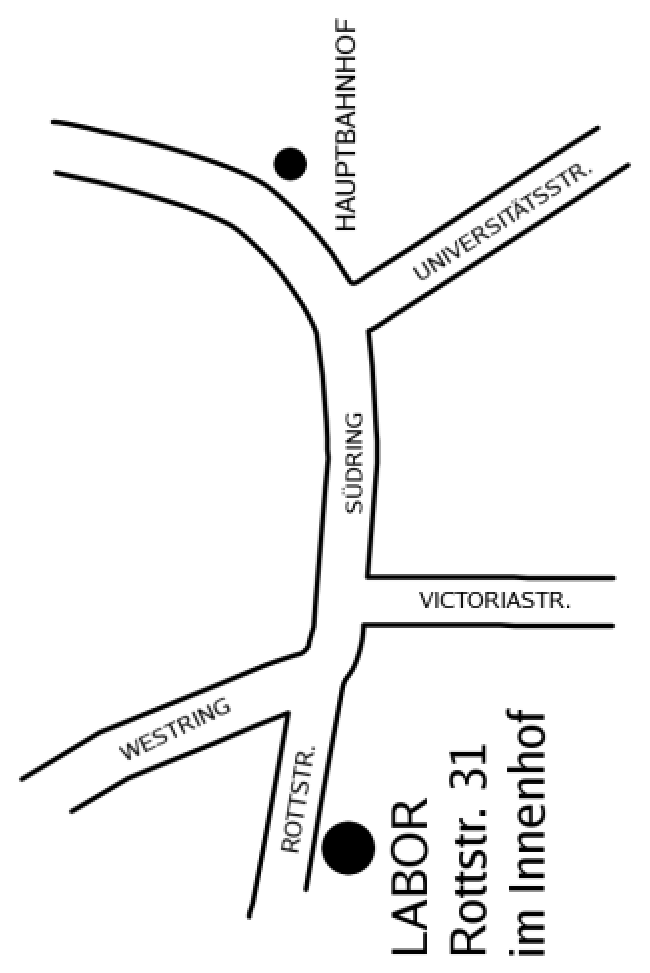
\includegraphics[width=45mm,angle=270]{images/anfahrt.epsi}
\end{center}



\pagebreak




% ABOUT US
\section{\"Uber uns}

{\bf Konsumgewohnheiten vs. Rabattpunkte}\\
Alle Menschen verschenken ihre Privatsph\"are f\"ur ein paar
Merchandising-Artikel? Keiner versteht, dass Du nicht Deine
Konsumgewohnheiten f\"ur ein paar Rabattpunkte offenlegen m\"ochtest? Keiner
denkt dar\"uber nach, was man mit einer zentralen Fingerabdruckdatenbank
aller EU-B\"urger alles falsch machen kann? Keinen interessiert es, dass
jeder Informationsseitenabruf und -kontakt bald jahrelang gespeichert
wird? Denkst DU! Wir sollten uns dar\"uber unterhalten!\\
Dar\"uber, und auch \"uber Fragen wie "Kann das Konzept der
‘Kulturflatrate’ \"uberhaupt funktionieren oder stirbt die kulturelle
Vielfalt dann gleich mit?”, “Was bringen RFID- Erfassungsger\"ate an
Fußg\"angerampeln?”, "Wie k\"onnen offene B\"urgernetze als Alternative
zum Internet gestaltet werden?" oder auch “Kann man mit einem Trusted
Platform Module auch was Sinnvolles anfangen?“\\
\\
\begin{center}
\centering 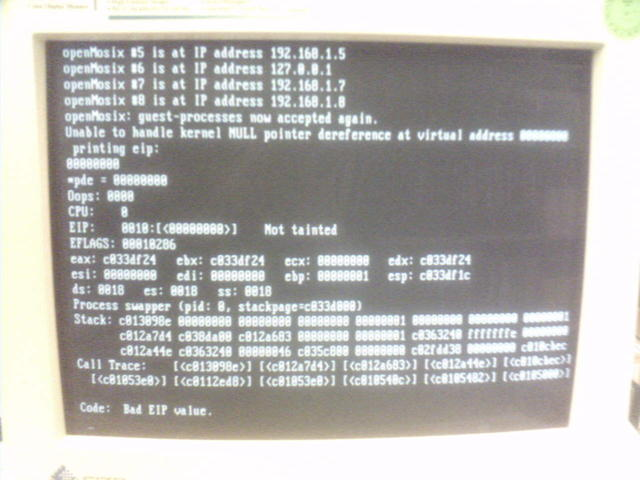
\includegraphics[width=60mm,angle=270]{images/eip.epsi}
\end{center}

\vskip 2cm

{\bf Wer bastelt hat Recht}\\
Das LABOR ist ein Ort, an dem in erster Linie gemacht und gedacht wird:
Wir benutzen und entwickeln freie Software; wir l\"oten, \"atzen und
programmieren Mikrocontrollerschaltungen; basteln Antennen; denken uns
praktikable L\"osungen f\"ur einen gesellschaftlichen Umgang mit vorhandener
oder sich entwickelnder Technik aus - wir haben den Anspruch mit Technologie
Neues und Sinnvolles zu gestalten.\\
Das LABOR ist dynamisch, seine Strukturen nicht fest. Was in und mit
ihm passiert, h\"angt auch von Dir ab. Du willst etwas ver\"andern oder
verbessern? Technik ausprobieren oder \"uber deren Einsatzm\"oglichkeiten
lernen? - Oder einfach nur Leute kennenlernen, die das auch tun? - Dann
komm' vorbei und mach mit - das LABOR entwickelt sich mit Dir!\\
{\bf Lerne die Regeln, damit du weißt, wie man sie bricht}\\
Wichtiger als Hardware und Equipment sind Menschen, die wissen, wie das alles
funktioniert. Im Labor gibt es Vortr\"age, Workshops und Diskussionen zu
den unterschiedlichsten Technologien. Wenn keine Veranstaltung stattfindet,
bastelt man - zusammen oder alleine. Aber immer tauscht man sein Wissen: Denn
alles, was Dir zeigt, wie die Welt funktioniert, hat hier seinen Platz.\\
\\
{\bf N\"achster Termin f\"ur Hereingucker}\\
Komm doch einfach zu einem unserer Open Meetings vorbei! Am besten n\"achsten
Mittwoch abends so ab 19.30 Uhr.\\

\vskip 2cm



% AUFMACHER

\begin{center}
\centering 
\includegraphics[width=60mm,angle=0]{images/logo.epsi}
\end{center}

\vskip 5mm

{\centering \huge Programm September 2006} % dyna

\vskip 5mm

Jetzt! Schnell! Terminkalender aufschlagen! In der Hand h\"altst du den
Veranstaltungskalender des LABORs. Du solltest besser mal reinschauen,
Dir einen Stift schnappen und Dir vormerken, wann DU vorbeischaust! \\
\\
Das LABOR ist Dein Raum in Bochums Innenstadt, in dem Platz ist f\"ur
Dinge, die Du zu Hause nicht tun kannst. Hier triffst Du andere Leute,
die mit Technik kreativ, konstruktiv und kritisch umgehen. Hier ist
Deine Infrastruktur, Dein WLAN, Dein L\"otkolben, Deine Bastelecke. Du
kannst Vortr\"age h\"oren, an Workshops teilnehmen, oder selber welche
veranstalten. Join us! \\

\begin{center}
\centering 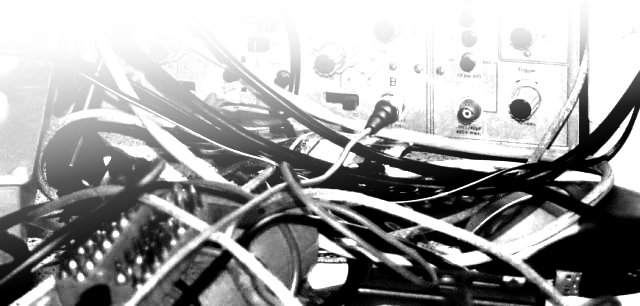
\includegraphics[width=30mm,angle=270]{images/kabel.epsi}
\end{center}


\end{multicols}
\end{document}
